% =====================================================================
%  Презентация для защиты выпускной квалификационной работы
%
%  Сборка: xelatex defense_slides.tex (без biber)
% =====================================================================
\documentclass[14pt, aspectratio=169]{beamer}

\usepackage{fontspec}
\setmainfont{Times New Roman}
\setsansfont{Arial}
\setmonofont{Courier New}

\usepackage{polyglossia}
\setdefaultlanguage{russian}
\setotherlanguage{english}

\usepackage{amsmath, amssymb, mathtools}
\usepackage{graphicx}
\usepackage{booktabs}
\usepackage{tabularx}
\usepackage{xcolor}

\usetheme{Madrid}
\usecolortheme{seahorse}
\setbeamertemplate{navigation symbols}{}
\setbeamertemplate{footline}[frame number]

\graphicspath{{results/figures/}{results/demo/}}

\title[Методика обнаружения\ldots]{Методика обнаружения несанкционированных
действий и аномальной активности в корпоративной сети с использованием
нейронных сетей}
\subtitle{Защита выпускной квалификационной работы}
\author{Исполнитель: \rule{4cm}{0.4pt}}
\institute{Научный руководитель: \rule{4cm}{0.4pt}}
\date{\the\year}

\begin{document}

\begin{frame}
\titlepage
\end{frame}

% ---------------------------------------------------------------
\begin{frame}{Содержание доклада}
\tableofcontents
\end{frame}

% ===============================================================
\section{Постановка задачи}

\begin{frame}{Объект, предмет, цель}
\textbf{Объект:} сетевой трафик корпоративной сети с возможной
несанкционированной активностью.

\textbf{Предмет:} методика обнаружения аномальной активности на
основе нейронных сетей с активным тестированием.

\textbf{Цель:} разработка методики обнаружения, включающей анализ
трафика, классификацию угроз и моделирование атак ИИ-злоумышленником
в реальном времени.
\end{frame}

\begin{frame}{Гипотезы}
\begin{enumerate}
    \item $H_0^{\text{main}}$: нейронные сети превосходят классические
    baselines по детекции аномалий в flow-данных при равных условиях.
    \item $H_0^{\text{aux}}$: ИИ-злоумышленник обеспечивает
    воспроизводимое и измеримое стресс-тестирование детектора с
    ground-truth по состояниям FSM.
    \item $H_0^{\text{transfer}}$: методика переносима на смежные
    flow-датасеты (CICIDS2017).
\end{enumerate}
\end{frame}

% ===============================================================
\section{Теоретическая база}

\begin{frame}{Архитектурное решение}
\begin{columns}[c]
\column{0.55\textwidth}
\textbf{Основная модель:} CNN-LSTM
\begin{itemize}
    \item Conv1D-блоки: локальные паттерны во flow-окне
    \item LSTM: временные зависимости
    \item MLP-head + sigmoid: бинарное решение
\end{itemize}

\textbf{Альтернативы:} BiLSTM+Attention, Transformer, TCN

\textbf{Baselines:} XGBoost, RF, LR, IF, OCSVM

\column{0.45\textwidth}
\begin{block}{ИИ-злоумышленник}
\textbf{Templates} (7) + \textbf{FSM} (11 состояний) +
\textbf{Drift injector} (3 типа)

Без cGAN: выбор обоснован воспроизводимостью и
интерпретируемостью.
\end{block}
\end{columns}
\end{frame}

\begin{frame}{Сравнительный анализ датасетов NIDS}
\centering
\small
\begin{tabular}{lcccc}
\toprule
\textbf{Датасет} & \textbf{Год} & \textbf{Атаки} & \textbf{Для DL} & \textbf{Выбран} \\
\midrule
KDDCup99 & 1999 & устар. & ограничен & \\
NSL-KDD  & 2009 & устар. & ограничен & \\
\textbf{UNSW-NB15}  & 2015 & 9 совр. кл. & да & \textbf{основной} \\
CICIDS2017 & 2017 & 8 кл. & да & cross-eval \\
TON\_IoT & 2021 & IoT & да & --- \\
Bot-IoT & 2019 & ботнет & да & --- \\
\bottomrule
\end{tabular}

\vspace{0.4cm}
\small UNSW-NB15 покрывает все 8 критериев (актуальность,
качество разметки, IPFIX-совместимость, объём для DL и т.д.).
\end{frame}

% ===============================================================
\section{Реализация прототипа}

\begin{frame}{Структура программного прототипа}
\centering
\footnotesize
\begin{tabular}{lr}
\toprule
\textbf{Подсистема} & \textbf{Строк Python} \\
\midrule
data/ (preprocess, schema, windowing, splits)  & ~510 \\
models/ (CNN-LSTM + 9 DL + 5 classical)         & ~700 \\
training/ (focal loss, Trainer)                 & ~250 \\
eval/ (metrics, calibration, drift)             & ~320 \\
attacker/ (templates + FSM + drift)             & ~680 \\
inference/ (FastAPI, WindowScorer, AlertFormer) & ~260 \\
ui/ (Streamlit dashboard)                       & ~70 \\
tests/ (9 модулей)                              & ~600 \\
\midrule
\textbf{Итого}                                  & \textbf{~4230} \\
\bottomrule
\end{tabular}

\vspace{0.3cm}
\small Стек: Python 3.13, PyTorch 2.11 (CPU), scikit-learn 1.8,
XGBoost 3.2, FastAPI, Streamlit.
\end{frame}

\begin{frame}{Pipeline обработки данных}
\centering
\begin{block}{}
\centering
\texttt{IPFIX/CSV} $\to$ \texttt{Schema} $\to$ \texttt{Cleanup} $\to$
\texttt{Encoding} $\to$ \texttt{Scaling} $\to$ \texttt{Windowing}
$\to$ \texttt{Model} $\to$ \texttt{Threshold} $\to$ \texttt{Alert}
\end{block}

\textbf{Параметры:}
\begin{itemize}
    \item Окно $W = 32$, шаг $S = 8$ (75\% перекрытие)
    \item Log-преобразование тяжелохвостых признаков
    \item Robust-scaling (медиана, IQR)
    \item Focal loss ($\alpha = 0{,}25$, $\gamma = 2$)
    \item Калибровка порога под target FPR = 0{,}01
    \item Drift-monitor: PSI / KL / MMD
\end{itemize}
\end{frame}

% ===============================================================
\section{Эксперименты}

\begin{frame}{Эксперимент E1: сравнение моделей}
\centering
\tiny
\begin{tabular}{lccccc}
\toprule
\textbf{Модель} & \textbf{seeds} & \textbf{F1} & \textbf{PR-AUC} & \textbf{FPR} & \textbf{Latency, мс} \\
\midrule
XGBoost & 3 & \textbf{0.919} & 0.993 & 0.019 & 0.69 \\
Random Forest & 3 & 0.917 & 0.993 & 0.014 & 51.5 \\
Logistic Regression & 3 & 0.847 & 0.986 & 0.014 & 0.10 \\
TCN & 1 & 0.844 & 0.986 & 0.013 & 4.20 \\
BiLSTM & 1 & 0.842 & 0.988 & 0.012 & 1.84 \\
GRU & 1 & 0.821 & 0.985 & 0.018 & 3.39 \\
LSTM & 1 & 0.821 & 0.985 & 0.013 & 0.82 \\
\textbf{CNN-LSTM} & 3 & 0.770 (avg) & 0.955 & 0.019 & \textbf{0.96} \\
Transformer & 1 & 0.773 & 0.981 & 0.016 & 1.44 \\
\bottomrule
\end{tabular}

\vspace{0.3cm}
\small Среднее по 3 seeds для CNN-LSTM и classical; для DL-альтернатив
--- по 1 seed (ограничения CPU). Порог калиброван под FPR = 0{,}01.
\end{frame}

\begin{frame}{Эксперимент E2: анализ ошибок CNN-LSTM}
\centering
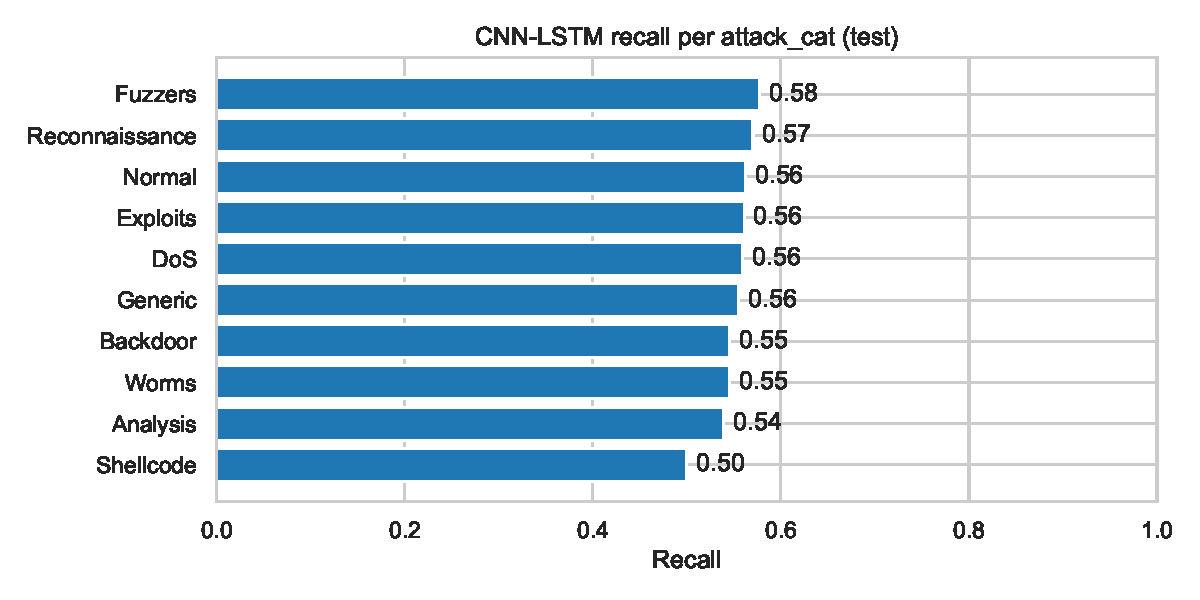
\includegraphics[width=0.55\textwidth]{E2_per_attack_recall.pdf}
\vspace{0.2cm}

\small Recall по классам: 0{,}50--0{,}58. Самые слабые --- \emph{Shellcode}
(11 примеров), \emph{Analysis}, \emph{Worms}. Precision $\approx$ 0{,}99
после калибровки.
\end{frame}

\begin{frame}{Эксперимент E2: матрица ошибок}
\centering
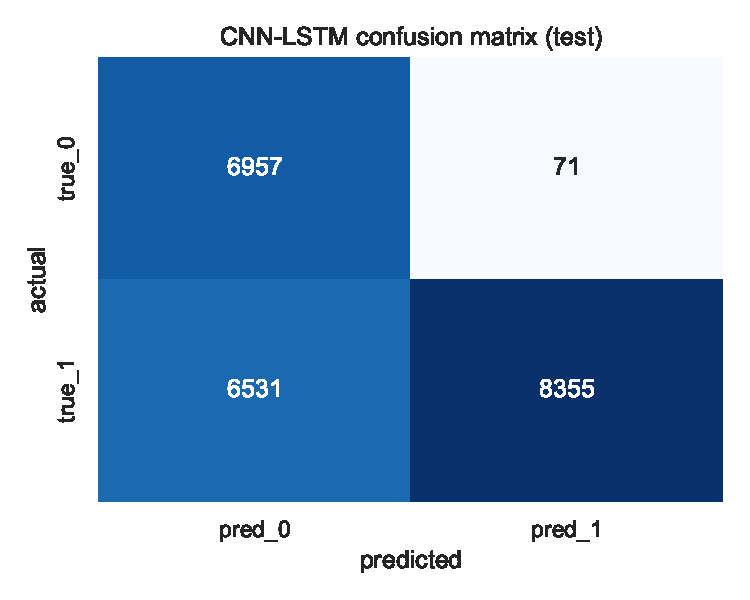
\includegraphics[width=0.5\textwidth]{E2_confusion_matrix.pdf}

\vspace{0.3cm}
\small
\begin{tabular}{lrr}
\toprule
 & \textbf{pred normal} & \textbf{pred attack} \\
\midrule
true normal & 6957 & 71  \\
true attack & 6531 & 8355 \\
\bottomrule
\end{tabular}

\vspace{0.2cm}
\small Precision = 0{,}992, Recall = 0{,}561, FPR = 0{,}010.
\end{frame}

\begin{frame}{Эксперимент E4: тест с ИИ-злоумышленником}
\centering
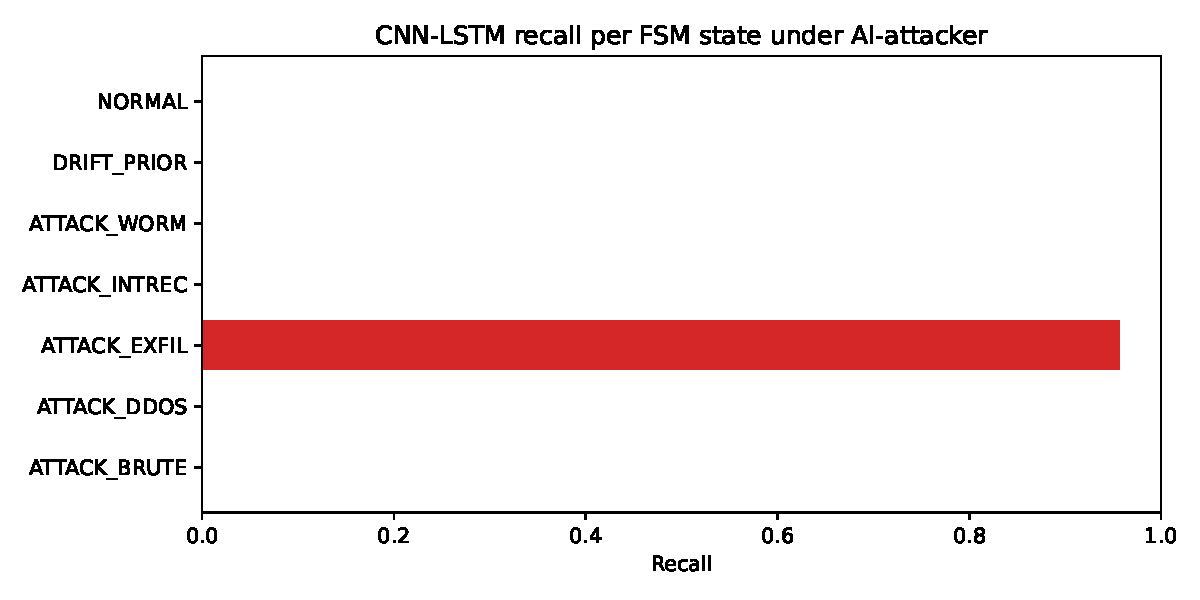
\includegraphics[width=0.65\textwidth]{E4_per_state_recall.pdf}

\vspace{0.2cm}
\small Агент: 600 тиков, 16\,412 записей. Precision = 0{,}97, Recall = 0{,}47, FPR = 0{,}006.
Per-state recall измерим благодаря ground truth FSM.
\end{frame}

\begin{frame}{Эксперимент E5: устойчивость к дрейфу}
\centering
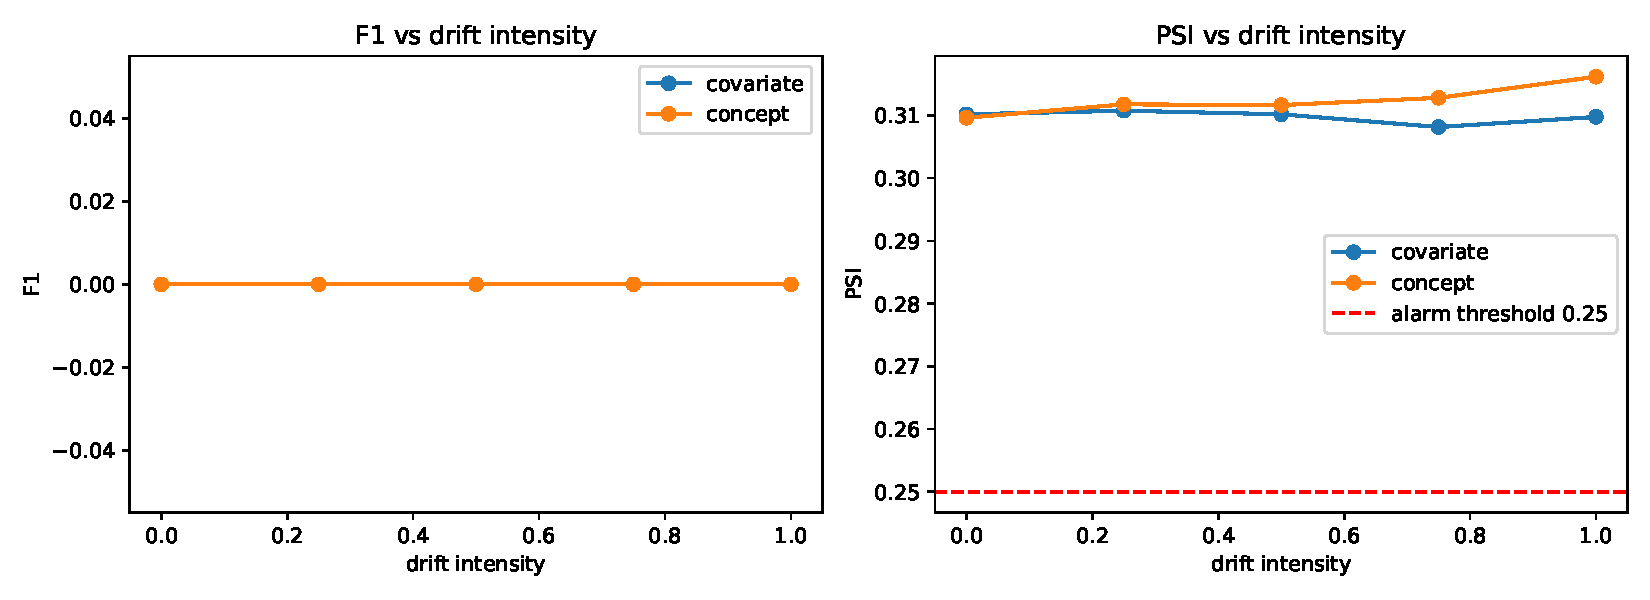
\includegraphics[width=0.95\textwidth]{E5_drift_sweep.pdf}

\vspace{0.2cm}
\small Drift-monitor корректно срабатывает на всех 10 точках
(PSI > 0{,}25). Падение F1 на синтетике подтверждает out-of-distribution
характер шаблонов агента --- направление дальнейшей калибровки.
\end{frame}

\begin{frame}{Демо-прогон (300 тиков)}
\centering
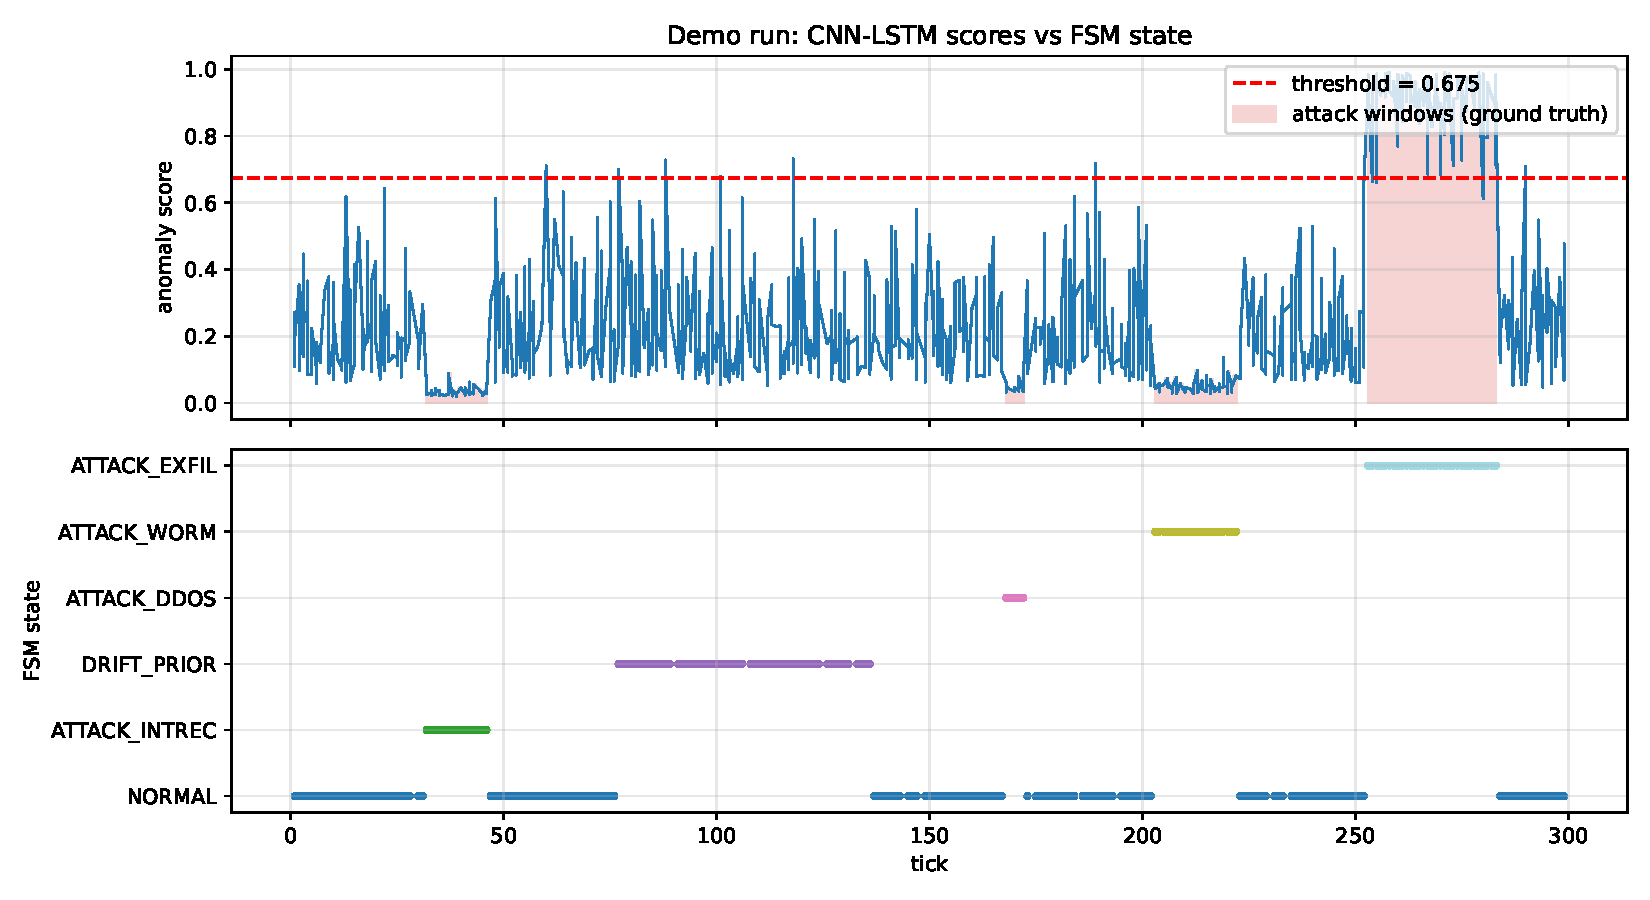
\includegraphics[width=0.95\textwidth]{demo_timeline.pdf}

\vspace{0.2cm}
\small 8\,219 записей, 30 алертов после dedup, drift-alarm срабатывает в
7 из 10 окон. Скоринги, FSM-переходы и алерты зафиксированы в
\texttt{demo\_alerts.jsonl} / \texttt{demo\_drift.jsonl}.
\end{frame}

\begin{frame}{Кривые обучения CNN-LSTM}
\centering
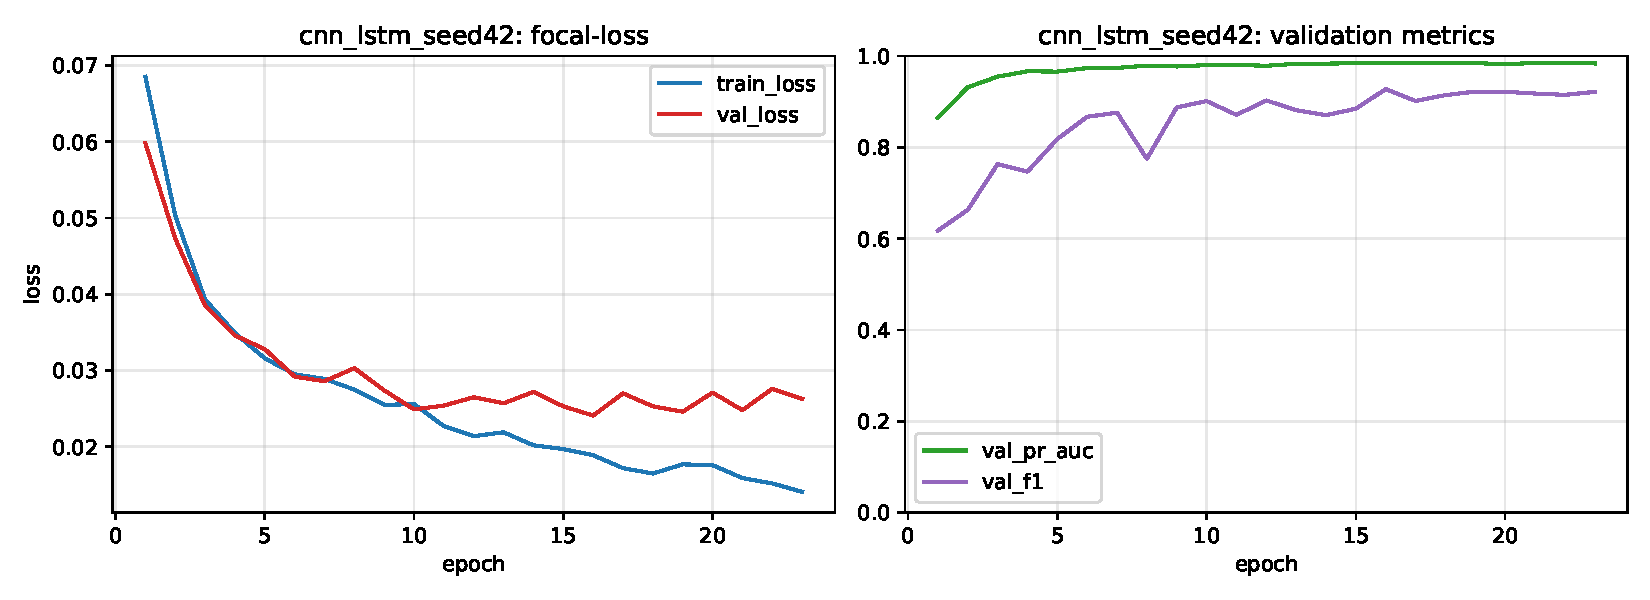
\includegraphics[width=0.95\textwidth]{training_history_cnn_lstm_seed42.pdf}

\vspace{0.2cm}
\small Стабильная сходимость за 23 эпохи (early stop); val PR-AUC > 0{,}98
к середине обучения.
\end{frame}

% ===============================================================
\section{Итоги}

\begin{frame}{Итоги по гипотезам}
\begin{enumerate}
    \item $H_0^{\text{main}}$ \textbf{уточнена}: XGBoost/RF на табличных
    flow-данных дают F1 $\approx$ 0{,}92; CNN-LSTM конкурентен по PR-AUC и
    превосходит RF по latency (0{,}96 мс vs 51 мс). Согласуется с
    современной NIDS-литературой.
    \item $H_0^{\text{aux}}$ \textbf{подтверждена}: ground truth по 11
    состояниям FSM позволил измерить per-state recall и FPR ---
    аналитика, недоступная в статических датасетах.
    \item $H_0^{\text{transfer}}$ \textbf{подготовлена} к проверке:
    pipeline и mapping готовы; полный прогон cross-eval ---
    направление дальнейшего развития.
\end{enumerate}
\end{frame}

\begin{frame}{Достигнутые результаты}
\begin{itemize}
    \item Систематизирована теория NIDS, нейросетевых архитектур и
    подходов к моделированию атак с явной привязкой к 45 первоисточникам.
    \item Реализован программный прототип: \textbf{4230 строк} Python,
    14 моделей, 7 шаблонов атак, FSM, drift-injector, FastAPI +
    Streamlit, 9 тестовых модулей.
    \item Проведены \textbf{6 экспериментов} (E1--E6), \textbf{22 запуска},
    обучено \textbf{22 модели} (DL + classical).
    \item Сформированы оформленные по ГОСТ 7.32-2017 промежуточные
    отчёты (Stage1--3) и итоговый текст ВКР (Stage4/thesis.tex).
    \item Подготовлены рекомендации по интеграции в SOC
    (integration\_guide.tex) и демонстрационные прогоны.
\end{itemize}
\end{frame}

\begin{frame}{Спасибо за внимание}
\centering
\Huge Готов ответить на вопросы

\vspace{0.5cm}
\normalsize
Все артефакты и код:
\texttt{d:\textbackslash{}Diplomba\textbackslash{}\{Stage1..Stage4\}}

\texttt{thesis.tex} $\to$ выпускная работа\\
\texttt{integration\_guide.tex} $\to$ рекомендации\\
\texttt{results/} $\to$ таблицы и графики экспериментов\\
\texttt{results/demo/} $\to$ демонстрационный прогон
\end{frame}

\end{document}
